\begin{figure*}[h]                                                           
 
\includegraphics[width=0.95\linewidth]{./media/images/world_iguana}%
  \scriptsize{\textsc{\\topic modeling lightens} the burden of creating complete works of IF}
  \label{fig:editorial}%                                                 
\end{figure*}                                                                

\begin{quotation} 
  \noindent\color{Sepia}{\textit{\textbf{“Writing is an exploration. You start from nothing and learn as you go.”}}}\\[.5mm]
   \hfill\color{Sepia}{\small{\textendash E. L. Doctorow}}
\end{quotation} 
%\begin{abstract}
%\textbf{\emph{“In the beginning the Universe was created. This has made a lot of people very angry and been widely regarded as a bad move.”  \\ \\--- Douglas Adams}}
%\end{abstract}
\newpage
\marginnote{\href{https://www.analyticsvidhya.com/blog/2016/08/beginners-guide-to-topic-modeling-in-python/}{Shivam Bansal, Beginners Guide to Topic Modeling Modeling in Python}}[2em]
\lettrine[lines=3]{\color{BrickRed}L}{\enspace et's explore how to}
gain a foothold on our project's topic relationships
using\textsc{gensim}. Once you've determined what your work of \textsc{if} is about
it would be nice to discover what kind of related areas we can find and how all these topics tie together.

\section{relationships to diagrams} \label{sec:relations}
When we're finished, we'll be able to query the entire work of
Wikipedia about virtually any topic imaginable. Here's what a query for
\textit{Temple of Athena Nike} looks like:
\begin{lstlisting}
\$ python run_search.py
Loading Wikipedia LSI index (15-30sec.)...
   Loading LSI vectors took 2.53 seconds

Loading Wikipedia article titles...

Searching for articles similar to
'Temple of Athena Nike':
    Similarity search took 1434 ms
    Sorting took 4.40 seconds

Results:
    Temple of Athena Nike
    Temple of Poseidon at Sounion
    Temple of Hera, Olympia
    Temple of Artemis, Corfu
    Athena Alea
    Temple of Olympian Zeus, Athens
    Temple F (Selinus)
    Bassae
    ...
  \end{lstlisting}
  %Author's image
%  \begin{wrapfigure}{l}{.15\textwidth}
%    \begin{center}
%      \parbox{.15\textwidth}{
%        \includegraphics[width=.15\textwidth, keepaspectratio=true]{../images/ center_top_one_one.svg} \href{http://www.commondreams.org/author/nadia-prupis-staff-writer}{{\small{\textbf{By Nadia Prupis}}}} }
%    \end{center}
%  \end{wrapfigure} \\

  Notice that the topic modeller returns a list of related topics by order of
  relevance. The topic modeler is not a search engine\textemdash it's core
  purpose is not to \textit{match} your inquiry; its purpose
  is to return items \textit{closely related} to your inquiry. By providing
  lists of closely related topics, you can quickly map the
  results to items of exploration in your work of \textsc{if}.

  Let's take another example. First, I'll start with a known article in Wikipedia
  by looking it up
  manually.\marginnote{\href{https://en.wikipedia.org/wiki/Platonic_realism}{Base
      topic, 'Platonic Realism'}} Topic modelling is not limited to physical
constructs, and this time I'd like this time to quickly see what areas are related to
Plato's idea of realism:
\pagebreak
\begin{lstlisting}
...
Searching for articles similar to
'Platonic realism':
...
Results:
    Platonic realism
    Ontology
    Indeterminacy (philosophy)
    Theory of forms
    A priori and a posteriori
    Schema (Kant)
    Substance theory
    Nominalism
    ...
\end{lstlisting}
From here I can choose Ontology, the study of being, as a preamble to my
adventure. The interlocutor could prove that
they understand Ontology before moving to the next phase of adventure. Once they
do the room lights up to reveal a being manifested physically in the updated,
brightly lig room description.

I point a summarizer to the \emph{Platonic realism} topic:

\begin{lstlisting}
sumy lex-rank --length=5 --url https://en.wikipedia.org/wiki/Platonic_realism
\end{lstlisting}

\begin{quote}
In Platonic realism, forms are related to particulars (instances of objects and properties) in that a particular is regarded as a copy of its form.
\end{quote}
I point a summarizer to the Ontology topic:

\begin{lstlisting}
sumy lex-rank --length=5 --url https://en.wikipedia.org/wiki/ontology
\end{lstlisting}

\begin{quote}
This view allows philosophical entities other than actual entities to really exist, but not as fundamentally and primarily factual or causally efficacious; they have existence as abstractions, with reality only derived from their reference to actual entities.
\end{quote}

\includepdf[scale=1.01]{media/images/pepper.pdf}
And finally to the second most relevant result,
\emph{Indeterminancy\_(philosophy)} topic just for fun:
\begin{lstlisting}
sumy lex-rank --length=5 --url 'https://en.wikipedia.org/wiki/Indeterminacy_(philosophy)'
\end{lstlisting}
\begin{quote}
Science generally attempts to eliminate vague definitions, causally inert entities, and indeterminate properties, via further observation, experimentation, characterization, and explanation.
Chaos theory argues that precise prediction of the behavior of complex systems becomes impossible because of the observer's inability to gather all necessary data.
\end{quote}
\marginnote{
\label{lst:relationships}
The Graphiz graphing file \textattachfile{media/images/relationships.dot}{\color{red!50!black}{\emph{relationships.dot}}} is attached to this document (if your reader supports it) and is also \hyperlink{lst:relationships}{listed in the end notes}.
}[1em]
\pagenote[Page \pageref{lst:relationships}, Graphiz relationship graph code
listing]{\hypertarget{lst:relationships}{\lstinputlisting{media/images/relationships.dot}}
}
\noindent We can now graph the results using the Graphiz language \textemdash I see that the Indeterminacy topic mentions
'Foucault,' author of ``The Archeology of Knowlege,'' so we'll throw in
what he has to say about Indeterminacy. In a
few minutes, we get this relationship graph with the source file:
\begin{landscape}
\begin{figure*}[ht]                                                           
  \centering
  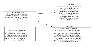
\includegraphics[width=\linewidth]{./media/images/graph}
  \caption{\textsc{entity relationship graph} graph drawn using the results of
    topic modelling.}
  \label{fig:editorial}%                                                 
\end{figure*}                                                                
\end{landscape}
\section{topic modeling preparation}
Here are the steps to create the topic modelling system:
\begin{enumerate}
  \item Downloading a complete record of all Wikipedia articles (i.e. a
    ``dump'')
  \item Converting articles to a ``big bag of words''
  \item Learning ``term-frequency–inverse document frequency'' \textsc{[tf-idf]} from bag of words
  \item Applying \textsc{tf-idf} model to all vectors
  \item Formulating a Latent Semantic Index \textsc{[lsi]} via shallow artificial neural network
    \item Applying \textsc{lsi} to all vectors
\end{enumerate}
Fortunately, a script is available \marginnote{\href{https://www.kdnuggets.com/2017/12/general-approach-preprocessing-text-data.html}{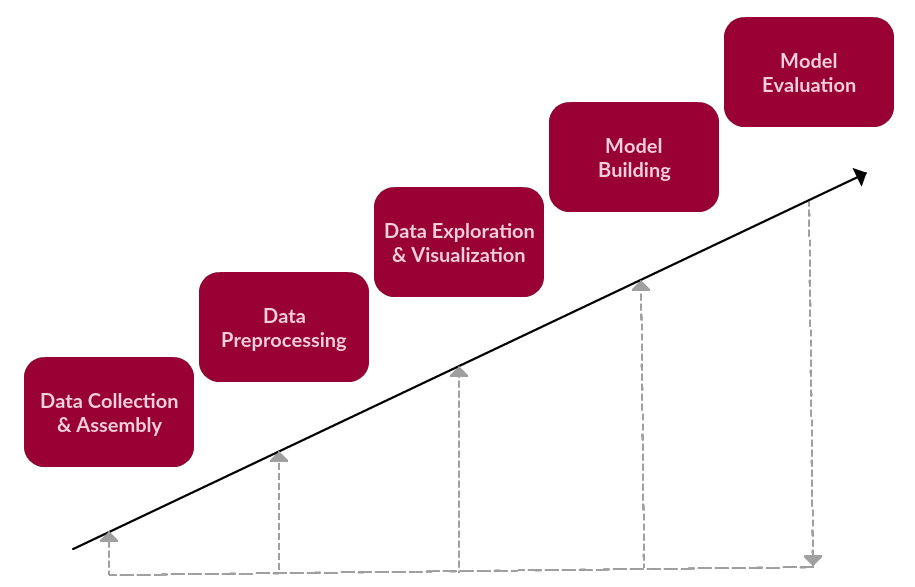
\includegraphics[width=\linewidth]{media/images/framework}\\
    Matthew Mayo, ``A General Approach to Preprocessing Text Data''}} that performs all these steps for you. Once
you've installed the necessary requirements to your system (outlined below)
you'll be ready to run the topic modeling queries as shown beginning on page
\pageref{sec:relations}. For effective topic modelling you needn't know the
details of the process.

\subsection{installing prerequisites}
\textsc{gensim} requires \textsc{python, numpy, scipy, six, and smart\_open} to run.
Fortunately, either your operating system has a pre\textendash defined package
to install that will install all these dependencies for you or \textsc{python}'s
internal \textsc{pip} installation system will install the required dependencies
for you.

Installing \marginnote{\href{https://radimrehurek.com/gensim/install.html}{\textsc{gensim} quick install guide}}[2em] from your operating system's package manager is the preferred route; it will avoid conflicts down the road. On Arch Linux, for example, the command to install Gensim through \textsc{yaourt} is:
\begin{lstlisting}
  yaourt gensim
\end{lstlisting}

\marginnote{\href{https://github.com/BurntSushi/nfldb/wiki/Python-&-pip-Windows-installation}{\textsc{python} \& \textsc{pip} Windows installation guide}}[1em]
If your system does not have a defined package for \textsc{gensim} simply
install \textsc{python} and \textsc{pip}. From there, install \textsc{gensim}
using \textsc{pip}.

If you have to install \textsc{gensim} through \textsc{pip}\textemdash as slightly
preferred in my opinion because \textsc{pip} generally provides recent versions\textemdash then
\textsc{gensim} may be installed by executing:

\begin{lstlisting}
pip install --upgrade gensim
\end{lstlisting}
\subsection{good citizenry: downloading wikipedia}
Now that \textsc{gensim} and its pre\textendash requisites are installed, we can
use these tools to download \& prepare the Wikipedia article dump
for use.

The Wikipedia article dump is big, taking around 15\textsc{gb} and growing. The
preferred way to download the dump is through a torrent file. Torrent downloads
reduce the load on a server by spreading the bandwidth use across multiple servers. The
second\textendash most preferred way is to download the dump from a Wikipedia mirror. The least
preferred way is to download the dump from Wikipedia's server proper.

Wikipedia dump file names are in the form:
\begin{lstlisting}
  enwiki-[latest]-pages-articles.xml
  \end{lstlisting}
Download the latest torrent file ({\small enwiki-20170820-pages-articles.xml.bz2} as of
this writing) to your normal download directory.

Fire up your torrent client,
\marginnote{\href{https://harbhag.wordpress.com/2010/06/30/tutorial-using-rtorrent-on-linux-like-a-pro/}{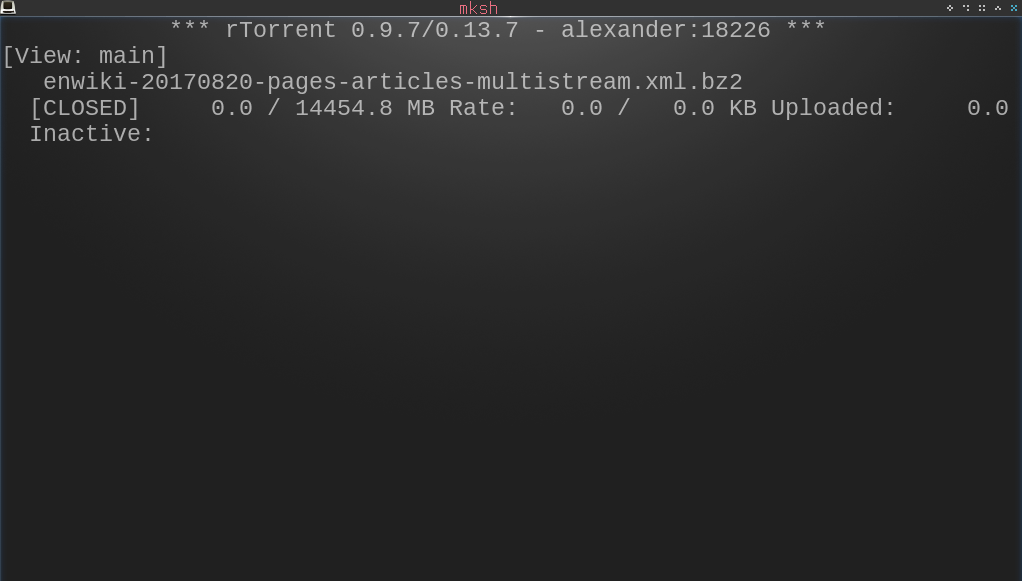
\includegraphics[width=\linewidth]{media/images/rtorrent}\\ \textsc{rtorrent}
  installation and use guide}} or double-click the torrent file you just
downloaded, and initiate the torrent download process. I personally used the
terminal\textendash based \textsc{rtorrent} but any torrent client will do. Be
patient; the Wikipedia dump is a large download and will take time to finish, even if your system is connected to fiber\textendash optic lines.
\subsection{downloading from a mirror}
Alternatively, you can download the dump from a
mirror.\marginnote{\href{https://dumps.wikimedia.org/mirrors.html}{Wikipedia
    Mirror List}}[2em] These are generally \textsc{ftp} sites. The key to finding the file you want is to navagate to the \textit{enwiki} subdirectory.
An example \textsc{url} looks like this:
\begin{lstlisting}
http://ftp.acc.umu.se/mirror/wikimedia.org/dumps/enwiki/20180901/enwiki-20180901-pages-articles.xml.bz2
\end{lstlisting}
Once you've selected the appropriate file, click the link and download as you normal.

\subsection{installing wiki\textendash sim\textendash search} \label{sec:wikisim}
\textsc{wiki-sim-search} is a python script \marginnote{\href{https://github.com/chrisjmccormick/wiki-sim-search}{\textsc{wiki\textendash sim \textendash search} Github repository, including instructions for use}}
that automatically processes the
Wikimedia articles into forms usable for topic modeling with \textsc{gensim}. To
install \textsc{wiki-sim-search} you can either download the zip file or project's
repository using \textsc{git}. 

Once \textsc{wiki-sim-search} is cloned or decompressed, copy (or move) the
\texttt{\small{enwiki-[latest]-pages-articles.xml.bz2}} to the \texttt{data} directory
of the project.

Once the Wikipedia articles are in place, run this to process the Wikipedia dump:
\begin{lstlisting}
python make_wikicorpus.py
\end{lstlisting}
It will take roughly 12 hours on an
\textsc{intel i7}. The process, at least on \textsc{linux}, will not seem to be doing
anything. Be patient\ldots if you see the cursor just blinking when the program
hasn't returned an error it is running and should finish. The output will look
similiar to this:
\begin{lstlisting}
Parsing Wikipedia to build Dictionary...
    Building dictionary took 3:05
    8746676 unique tokens before pruning.

Converting to bag of words...
    Conversion to bag-of-words took 3:47

Learning tf-idf model from data...
    Building tf-idf model took 0:47
     
Applying tf-idf model to all vectors...
    Applying tf-idf model took 1:40

Learning LSI model from the tf-idf vectors...
    Building LSI model took 2:07

Applying LSI model to all vectors...
    Applying LSI model took 2:00
\end{lstlisting}
You may get a print statement error immediately after running
\textsc{make\_wikicorpus.py} like this:
\marginnote{\href{https://docs.python.org/3/whatsnew/3.0.html\#print-is-a-function}{Changed print statement in Python 3.0}}[2em]
\begin{lstlisting}
  File "make_wikicorpus.py", line 80
    print 'Parsing Wikipedia to build Dictionary...'
SyntaxError: invalid syntax
\end{lstlisting}
This error occurs when you are running the latest version of python. Go into the
\texttt{make\_wikicorpus.py} file and add parenthesis to every print statement.
For example, change the print statement from this:
\begin{lstlisting} 
  print 'Parsing Wikipedia to build Dictionary...'
\end{lstlisting}
To this:
\begin{lstlisting}
  print ('Parsing Wikipedia to build Dictionary...')
\end{lstlisting}
\marginnote{\href{https://nlpforhackers.io/topic-modeling/}{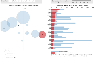
\includegraphics[width=\linewidth]{media/images/gensim_graph}\\
    Topic Modeling with \textsc{gensim} affords several ways to find and
    analyise topics and key word relationships}
} Adding parentheses to print statements also applies to the other search functions: \textsc{simsearch.py}, \textsc{keysearch.py}, and \textsc{searchwithwimwearch.py}.

Once the \textsc{make\_wikicorpus.py} function finishes you'll be ready to run
topic modeling as described at the beginning of this article. To search for a
specific topic, change the \textsc{query\_title} variable in line 29 of the
\textsc{run\_search.py} file to your topic of choice.

For example, change line 29 from this:
\begin{lstlisting}
query_title = 'Topic model'
\end{lstlisting}
To this:
\begin{lstlisting}
query_title = 'Platonic realism'
\end{lstlisting}
The ``trick'' is to search for Wikipedia articles titles proper using case
sensitive queries. To run the search again on one of the results, copy \&
paste the result and modify \textsc{run\_search.py}'s \texttt{query\_title}
variable.

Here you have it\textemdash a method for quickly pulling in topic relationships
for whatever your project calls for. By using Wikipedia as a base you are
pulling from a large ``real\textemdash world'' body of information. Even if you
model your topics loosely against the wikipedia corpus (perhaps ``Josh Wayne'' in your story is
closely modeled after ``John Wayne''), your stories
will ``feel'' authentic because they are based on authentic sources.